%begin preamble
\documentclass[12pt]{article} 
\setlength\parindent{0pt}
\renewcommand{\vec}[1]{\mathbf{#1}}

%packages
\usepackage{amsmath} % AMS Math Package
%\usepackage{siunitx} % si units
\usepackage{amssymb}	% Math symbols such as \mathbb
\usepackage{multicol} % Allows for multiple columns
\usepackage[small]{caption}%small captions
\usepackage{enumerate}%custom enumerations
\usepackage{enumitem} 
\usepackage{graphicx,epstopdf}
\usepackage{sectsty}
\usepackage{titlesec}
\usepackage[dvips,a4paper,top=1.54cm,bottom=3.25cm,left=3cm,right=3cm]{geometry}%margins and paper size
%end package

%cover page command
\newcommand{\makecover}[9]{
\thispagestyle{empty}
\setcounter{page}{0}
\begin{center}\LARGE{\bf #1}\vskip 24pt \normalsize{#2}\hspace*{\fill}\\
#3\vskip 12pt School of Physics and Astronomy\\The University of Manchester\vskip 12pt #4 Year MPhys Report\vskip 12pt
#5 \vskip 12pt
#6 \vskip 12pt
#7 \vskip 12pt
#8 \end{center}\section*{Abstract}

#9\newpage}

%end of coverpage command

\sectionfont{\normalsize\bfseries\fontfamily{ptm}\selectfont}
\subsectionfont{\normalsize\bfseries\fontfamily{ptm}\selectfont}
\subsubsectionfont{\normalsize\bfseries\fontfamily{ptm}\selectfont}

\pagestyle{plain}%page numbers in footer

%end preamble
\begin{document}

%Coverpage begin

%call \makecover with arguments: title, author, student id, year (first, second, third), date (mth year), partner name, abstract.
\makecover
{Discovering pulsars and transients with intelligent algorithms}
{Alex Lisboa-Wright}
{8928493}
{Fourth}
{May 2017}
{Project undertaken in collaboration with Lewis Smith (ID 8933715)}
{Project supervised by Dr Michael Keith}
{This is the final report of a full-year project}
{This project aimed to use intelligent algorithms to improve the detection of pulsars and fast radio bursts (FRBs). For pulsars, supervised-learning algorithms were used. A statistically significant improvement in the rate of discovery of real pulsars in the data was achieved, by adding simulated pulsars to the training data. For FRBs, unsupervised-learning algorithms, which were trained only on noise data, were assessed to be more useful due to the lack of representative FRB datasets. In particular, the Isolation Forest classifier was shown to be both time-efficient and effective in finding FRBs.}
%Coverpage end
\par

\section{Introduction}
\subsection{Pulsars and millisecond pulsars}
Pulsars are rotating neutron stars, formed during supernova (SN) explosions, whose magnetic axes are sufficiently aligned with the Earth that radiation from the magnetic polar regions can be detected. They have high rotation frequencies (low periods) due to conservation of angular momentum holding during the supernova event as the star radially sheds mass. Millisecond pulsars (MSPs) are a class of pulsars with unusually high frequency - high enough that they are thought to have gained additional angular momentum from a source other than the SN in which they are born, such as a companion star \cite{lorimer2008binary}.

\subsection{Fast radio bursts}
Fast radio bursts (FRBs) are transient (single-event) objects visible in the radio spectrum. They are characterised by short durations (less than 5 milliseconds) high signal-to-noise ratios (SNRs) and high dispersion measures (DMs) (see Section 3) after standard observational data processing, leading to their description as astrophysical sources of extragalactic origin. They are rare (18 confirmed as of the date of submission of this report, including a single repeating source \cite{scholz2016repeating}) and they can share similarities with terrestrial signals, including detections known as ``perytons", which were later found to be caused by radiation from a microwave oven \cite{petroff2015identifying}. These features combine to make FRBs extremely enigmatic and their discoveries difficult.

\subsection{Aims and motivation for the project}
The underlying aim of this year-long project was to explore ways of improving detection of pulsars, with a particular focus on MSPs, and fast radio bursts using intelligent algorithms. This field of study is motivated by the need for larger populations of confirmed pulsars and FRBs in order to better understand their underlying physics (and in the case of FRBs, their physical sources). As with other neutron stars, pulsars are useful as testing objects for general relativity, as markers of stellar populations due to their origin and for the physics of their degenerate neutron interiors and the structure associated with these. Due to the fractionally very small rate of change of the period between pulse signal for pulsars, any significant variations in the arrival times of the pulses, factoring in the motion of the Earth, are due to massive objects near the pulsar. This last application is especially relevant to MSPs. Fast radio bursts are of high interest in radio astronomy due to their unknown nature of their sources and the indication that the sources are located outside the Milky Way.
\paragraph{}
The Square Kilometre Array (SKA) is a series ofs array of dipole antennae and 15m-diameter radio dishes, covering a total area of circa 1km$^{2}$, which is currently under construction. Its purpose is to provide a much higher-resolution and higher-sensitivity radio picture of the sky, with myriad scientific objectives ranging all the way up to cosmological observations. It is due to come online within the next decade. The rate of data produced will be larger than that of the internet. Hence, storing all the SKA data will be impossible. Intelligent algorithms are being developed to classify data in real-time as it is collected by radio telescopes as data streams, with the SKA being the foremost application of this.
\paragraph{}
In this project, improvements to pulsar detection were attempted using observational datasets and features employed by previous research, simulating pulsar data points and combining these with the observational data to produce better training data for the intelligent algorithms. Improvements to FRBs involved finding a reliable set of features, given the lack of research, carried out using feature selection stability testing, and testing these features on real noise and simulated FRB data.

\subsection{The High Time Resolution Universe Survey}
HTRU is a survey conducted, initially using the Parkes Radio Telescope in Australia for the southern hemisphere, and later, the Effelsberg Radio Telescope in Germany for the northern hemisphere additionally from 2010 onwards \cite{keith2010high}\cite{ng2012conducting}, with the purpose of scanning the entire plane of the sky for pulsar and transient signals at the highest resolution used so far in the field. It uses multi-beam receivers to increase the resolution and observes at a radio frequency of 1.4 GHz.

\subsection{The GHRSS survey}
The GMRT High Resolution Southern Sky survey is a survey conducted with the Giant Metrewave Radio Telescope (GMRT) at a frequency of 322 MHz, for detecting pulsar and transient signals \cite{bhattacharyya2016gmrt}. Data recorded by this survey was used in this project as the noise data in the FRB datasets, to which simulated FRBs were added.

\section{Experimental background - astrophysical measurements}
This section summarises the main observational astrophysical quantities used in the experimental data, which are useful in distinguishing pulsars and FRBs from other sources of radio emission, such as radio frequency interference (RFI) or general astrophysical background emission. These quantities are the period of the emission (central to the pulse profile below), the signal-to-noise-ratio (SNR) and the dispersion measure (DM) measure. For FRBs, the relevant quantities are the DM, the SNR and the boxcar width.

\begin{figure}[h!]
\begin{center}
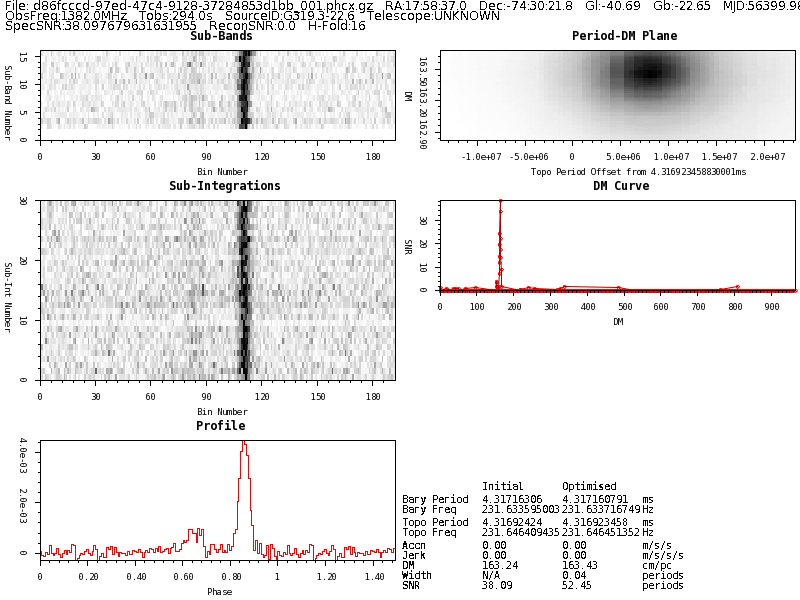
\includegraphics[scale=0.4]{d86fcccd-97ed-47c4-9128-37284853d1bb_001.png}
\caption{psrsoft image output for a simulated pulsar data file}
\label{psrsoftsim}
\end{center}
\end{figure}

\subsection{Pulse profile}
The pulse profile is a histogram of the average amplitude of the received radio emission as a function of the phase of an average pulse period. This profile is shown in the bottom left panel of Figure \ref{psrsoftsim}. By comparing the panels of the two figures, it is clear that a signal from a pulsar will have a more obvious curve (in red) and a clear peak or peaks (since the range of the phase extends beyond a single pulse, so the early part of the pulse repeats). Pilia et al. \cite{pilia2016wide}, using the LOw-Frequency ARray (LOFAR), demonstrate that there is a wide variety of pulse profile shapes, including multiple-peaked and heavily asymmetric profiles.

\subsection{Signal-to-noise ratio}
The SNR is simply the ratio of the power received from the source itself (the signal) versus that from other (background) objects, such as the cosmic microwave background (CMB), the atmosphere, the interstellar medium (ISM) or other origins (depending on the observing frequency). This could potentially include the telescope instrumentation. Readings with a higher SNR have a smaller relative error via signal averaging statistics, in which the SNR is proportional to the signal mean divided by the noise standard deviation. Therefore, higher SNRs are more likely to represent real source emission. The SNR can, however, be rendered less effective as a classification feature by RFI \cite{zhu2014searching} and must therefore be used in conjunction with other features when evaluating a source.

\subsection{Dispersion measure}
The dispersion measure (DM) is defined as the integral of the electron number density, $n_{e}$, over the line of sight to a given astronomical source \cite{ahuja2005tracking}:

\begin{equation}
\textnormal{DM} = \int_{0}^{L}n_{e}dl
\label{dm}
\end{equation}

where $L$ is the line-of-sight distance to the source. The unit of the DM is usually given as cm$^{-3}$pc. The DM is thus an electron column density, along the line-of-sight, between the observer and source. The DM is important because an ionized medium (such as the ISM), if situated along the line-of-sight, can cause the light emitted by the source to become dispersed by refraction or absorption and re-radiation, depending on the wavelength (and therefore the frequency) of the incident radiation. This causes a wavelength-dependent delay in the time at which the signal is detected. For two different frequencies, $f_{1}$ and $f_{2}$, this time delay is given in SI units by:

\begin{equation}
\Delta t= \frac{e^2}{2\pi mc}(f_{1}^{-2} - f_{2}^{-2}) \times \textnormal{DM}
\label{deltat}
\end{equation}

It is this frequency-dependent delay which is detected by the telescope's instrumentation, from which the DM is calculated. The DM is therefore an indicator of the amount of gas between an observer and a given source of emission. An example of the inverse square-law relation in Equation (\ref{deltat}) can be seen in Figure \ref{lorimerfrb}.

\begin{figure}[h!]
\begin{center}
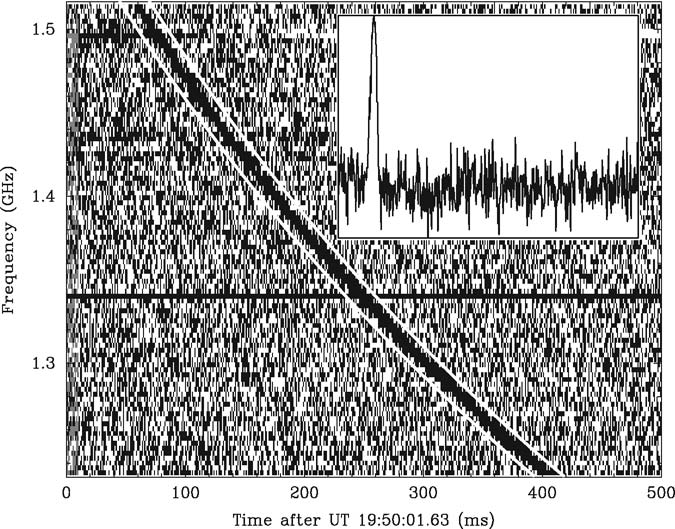
\includegraphics[scale=0.4]{lorimer_freq_vs_time.png}
\caption{Frequency-time plot for the Lorimer burst, the first confirmed FRB. Source:  \cite{lorimer2007bright}}
\label{lorimerfrb}
\end{center}
\end{figure}

\subsection{Boxcar width}
The boxcar width is essentially the time duration of a pulse of radio emission. A boxcar (top-hat) function is used as a smoothing function for the signal by convolving the pulse with the boxcar. Various widths of the boxcar function are tested, and the width taken forward is that which produces the highest SNR for the signal being studied. This width is treated as the duration of the signal.
\paragraph{}
This measure is important when searching for signal classes which are at least partially characterised by their duration - including FRBs, which last for less than 5 milliseconds. Boxcars are used in preference to Gaussian fits due to being much less complex mathematically while still providing reasonable accuracy for pulse duration estimation. This is highly advantageous in radio astronomy, where there are large quantities of received signals (from both astronomical and other sources) needing to be processed in even short observations.

\section{Data and pipelines}
\subsection{Pulsar data}
This project used the PulsarFeatureLab processing pipeline created by Lyon et al. \cite{lyon2016fifty} to process all data, including simulated data, to extract the desired features. It is designed to be compatible with various data file formats and has multiple output file type options. In addition, its feature extractor program can output any of a selection of feature groups, although it can be modified to take other feature sets as arguments.

\subsubsection{Observational data}
The observational pulsar datasets used for this project were:
\begin{itemize}
\item HTRU1: Dataset from HTRU processed by Morello et al. \cite{morello2014spinn}. Contained 74 classified MSPs, 1122 other classified pulsars and 89996 noise instances.
\item HTRU2: Dataset from HTRU processed by Lyon et al. \cite{lyon2016fifty} using PulsarFeatureLab. This was the principle test dataset in the pulsar part of the project. Contained 71 classified MSPs, 1568 other classified pulsars and 16259 noise instances.
\item LOTAAS: A dataset from the LOFAR Tied-Array All-Sky Survey (LOTAAS). This did not contain any classified MSPs and was therefore not useful for classification in this project.
\end{itemize}

%To check the applicability of the classification results.
\paragraph{}
In this project, MSPs and other pulsars (all treated during classification as being ``class 1") were distinguished by defining a threshold pulse period, below which classified pulsars were treated as MSPs and above which they were treated as non-MSPs. The definition described by Lorimer \cite{lorimer2008binary} of $P_{MSP}$ $\lesssim$ 30 ms was used as a guideline. The MSPs in the datasets, in order to include a few pulsars with periods slightly above 30ms, were defined as $P_{MSP}$ $\lesssim$ 31 ms. This maximised the number of MSPs, which were used as a testing set for the classifiers. Even so, there were very few examples of MSPs in the datasets, even relative to the number of other pulsars. For this project, the output pulsar data files were chosen to be in .arff (Attribute-Relation File Format) format in order to be compatible with the Waikato Environment Knowledge Analysis (WEKA) machine learning tool \cite{hall2009weka}. WEKA was used to visualise and count the different data types. The purpose of this was to find relationships between features to optimize the simulated pulsar data created during the project.
\paragraph{}
Candidates are classified by filtering out the most promising objects, then processing the data into graphical form (see Figure \ref{psrsoftsim}), which can be analysed by eye as having characteristics of a pulsar \cite{morello2014spinn}. Pulsars can be determined by a relatively narrow and dark vertical region in the sub-band and sub-integration panels, a relatively compact single dark region in the period-DM plane, a profile histogram that forms something that is approximately a continuous curve and a single DM-SNR peak, since the pulsar is a single source. Therefore, the object in Figure \ref{psrsoftsim} is a good example of a pulsar, while the object in Figure \ref{psrsoftnoise} (see Appendix) is clearly not. These images were generated using the psrsoft shell script \cite{thornton2013high}.
\paragraph{}
It was discovered that a significant fraction of the labelled millisecond pulsars (12 objects) in HTRU2 were not distinct pulsars. Instead, they proved to be one of the following:
\begin{itemize}
\item harmonics of detected pulsars (i.e. signals with integer multiples of the actual pulse frequency of the detected object), distinguished in psrsoft by having multiple lines in the sub-integration and sub-band plots and several peaks in their pulse profiles, all while having the same optimised SNR and DM outputs as the original detection.
\item RFI (i.e terrestrial inteference). This is characterised in psrsoft by a DM value that is  very small (usually \textless 10 pc cm$^{-3}$), as well as by a linear distribution of counts along a line of constant DM in the period-DM plane, indicating a signal with a continuous distribution of different periods and which is thus aperiodic.
\item a noise detection which displayed some, but not all, criteria used to define a pulsar by eye.
\end{itemize}

A few real objects also had unusual DM-SNR curves, in that their curves had far more points than other real objects, which changes the shape of the curves to appear less smooth (since the curve simply connects the plotted points, as shown in Figure \ref{psrsoftsim}) and therefore the relevant statistics. It was found that the observations in question were performed in the same observation season, so it was attributed to a change in the data-processing pipeline used only during that time period.

\subsubsection{Simulated MSP data}
The simulated pulsars were created with a random distribution of SNRs greater than 5 and uniform distibution of periods in the range of 5-20 milliseconds. This period range was chosen in order to coincide with the expected region of future MSP discoveries, especially MSPs which are easier to distinguish from non-MSP pulsars. The simulated pulse profiles were injected into real noise data files to make the curves more realistic than injecting them directly into the pipeline alone, as the curves would have benn far too smooth and therefore too easily separated from real data. To generate the final simulated data the injection was performed on a multiple-core GPU, due to the large processing power required. This produced a series of directories, each containing one simulated MSP data file and several noise files. The process used injection software provide by DSPSR \cite{van2011dspsr} and Tempo2 \cite{hobbs2006tempo2}.
\paragraph{}
Extraction of the simulated pulsar file was achieved by applying a score to each file. The score was a sum of the squares of the fractional deviations, of  both the pulse period and the DM value, from the original injected data values. Therefore, the pulsar file would ideally have a score of zero. However, the fitting during the process allowed the parameters to be adjusted, hence the need for the score. The program compared the scores within each directory and took the lowest score forward, subject a strict tolerance level of deviation from the original injected values. The tolerance for the frequency/period was selected to be the maximum size of the Doppler effect due to the orbital motion of the Earth, while the DM tolerance was set to be 0.7. The feature data was extracted and converted into ARFF format using PulsarFeatureLab.

\subsection{FRB data}

\begin{figure}[h!]
\begin{center}
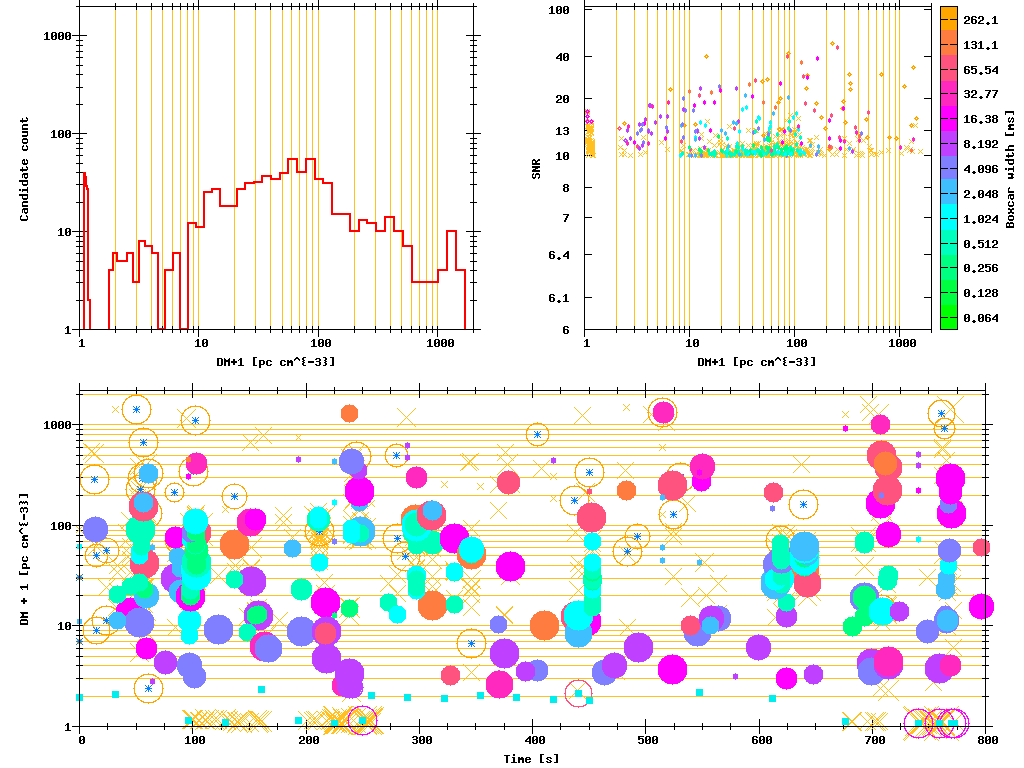
\includegraphics[scale=0.4]{HR_0222-44_injected.png}
\caption{Example of the Heimdall output}
\label{FRBheimdall}
\end{center}
\end{figure}

For training classifiers, given the small number of confirmed FRBs, the data was mostly observed noise, denoted as class-0 objects, together with simulated FRBs. The simulated FRBs were produced, injected into the data and then identified using the Heimdall pulse-detection code (\textsf{http://sourceforge.net/projects/heimdall-astro}) and injected into the noise data as class 1 objects. This gives data as shown in Figure \ref{FRBheimdall}. Each circle in the DM-time plot (bottom panel) represents a data point. The size of each of the circles in the figure is determines by the SNR of that particular data point and the colour indicates the optimal boxcar width of the data. As singular objects with small, FRBs might be expected to stand out as isolated points in the SNR-DM plot (top-right panel) and in the DM-time plot. Given the brief and transient nature of FRBs, they are unlikely to make an impression on the candidate count-DM plot (top-left panel).

\subsubsection{Feature selection}
Having obtained the data, it was then necessary to select the features to be used for classification. In particular, it was necessary to make a stable feature selection, i.e. select a set of features that is useful for classification of different training datasets. This was done by compiling a list of potential features, then applying these features to a group of similar (``perturbed") datasets to test their stability. These datasets were created from the dataset containing all relevant data by using k-fold cross validation. The value of $k$ was set to be 5 in order to maintain small perturbations between the datasets produced. The joint mutual information (JMI) of the features (see Section 4.1) was calculated for each dataset, and the features were ranked according to their JMI values, as before with the pulsar data. Then, the $n$ features with the highest JMI scores for each dataset are selected as the best feature set for that dataset, with $n < k$. For $k$ datasets and $f$ features, the objective is to produce the following matrix, $A$:
\[
A =
  \begin{bmatrix}
    \vec{s_{1}} \\
    \vec{s_{2}} \\
    .	\\
    :	\\
    \vec{s_{k}} \\
  \end{bmatrix}
  =
  \begin{bmatrix}
    x_{1,1} & x_{1,2} & ... & x_{1,f} \\
    x_{2,1} & x_{2,2} & ... & x_{2,f} \\
    .	    & .       & 	& .       \\
    :		& :		  &		& :	      \\
    x_{k,1} & x_{k,2} & ... & x_{k,f} \\
  \end{bmatrix}
\]
where for all $i$ and $j$, $x_{i,j} \in [0,1]$, i.e. the elements of $A$ are binary. If $x_{i,j} = 1$, the $j$th feature in the $i$th dataset has a JMI score which is in the top $n$ values for the $i$th dataset, and is "selected" \cite{nogueira2016measuring}. Otherwise, the element is zero and is not selected. The objective of creating this matrix is to check the similarity of all the individual rows (which are the results from each dataset) - a stable feature selection will produce a matrix of identical rows. Otherwise, small perturbations in data will directly affect the suitability of features, rendering the selection unstable, which is potentially catastrophic for observational searches for FRBs. This is shown in the example below, with $n = 2$, $f = 3$ and $k = 3$. Note the difference between rows in $A_{stable}$, which are identical, and $A_{unstable}$, where each dataset returns a different optimal set of features:
 \[
A_{stable} =
  \begin{bmatrix}
    1 & 1 & 0 \\
    1 & 1 & 0 \\
    1 & 1 & 0 \\
  \end{bmatrix}
, A_{unstable} =
  \begin{bmatrix}
    1 & 1 & 0 \\
    1 & 0 & 1 \\
    0 & 1 & 1 \\
  \end{bmatrix}
\]

There are a variety of causes for instability in feature selection - it can be due to one or more of the following:
\begin{itemize}
\item the datasets may vary significantly, such as one dataset having all the FRBs or many more high-SNR noise data points. This may cause some features to be significantly more or less effective. The value of k must be chosen carefully, therefore, to avoid this scenario while also being large enough to test the feature selection stability for other weaknesses.

\item a number (very close to, or greater than, the value of $f-n$) of the features given to the JMI calculator may produce very small JMI scores which are sensitive to random fluctuations over repeated runs. To solve this problem requires a large number of features which give JMI scores high enough to avoid fluctuations becoming significant. It should be noted that the available data must enable such features to be used - this is not guaranteed to be the case.

%\item
\end{itemize}

While stability can be visualized, particularly in simple cases like the above example, it must be quantified in order to be useful. This requires numerical similarity measures or functions, $\phi$, such that the overall stability measure, $\hat{\Phi}_{A}$, can be calculated via:

\begin{equation}
\hat{\Phi}_{A} = \frac{1}{k(k-1)} \sum\limits_{i=1}^{k}\sum\limits_{j=1, j \neq i}^{k}\phi(\vec{s_{i}}, \vec{s_{j}})
\end{equation}

Nogueira and Brown (2016)\cite{nogueira2016measuring} list the properties of an ideal $\phi$ function in the general case and compare them with those of functions currently in use. Following their recommendations with regard to these properties, the Pearson correlation coefficient was used to define $\phi$ as follows:
\begin{equation}
\phi_{Pearson}(\vec{s_{i}}, \vec{s_{j}}) = \frac{\sum\limits_{m=1}^{f}(x_{i,m} - \bar{x}_{i})(x_{j,m} - \bar{x}_{j})}{\sqrt{\sum\limits_{m=1}^{f}(x_{i,m} - \bar{x}_{i})^{2}} \sqrt{\sum\limits_{m=1}^{f}(x_{j,m} - \bar{x}_{j})^{2}}}
\end{equation}

where $\bar{x}_{i} = n/f$ It should be noted that $\phi_{Pearson}$ has a lower boundary of -1, not 0. However, it does returns 0 for a completely unstable (random) FS process, as required.

\iffalse
These are:
\begin{itemize}
\item \textbf{The stability measure must be fully defined.} Sometimes, a procedure is set up such that the number of features it selects is not always the same, a scenario for which some measures do not function properly.
\item \textbf{The measure must have finite upper and lower bounds.} It would be ideal for these bounds to be normalized to 0 (for maximum instability) and 1 (for maximum stability), respectively.
\item \textbf{Deterministic selection invariably leads to maximum stability, and vice versa.} If the same $n$ features are returned in every run, the measure should return its maximum value. The reverse should also apply.
\item \textbf{The value of the stability measure is independent of randomness in feature selection.} For completely random FS, the value of the measure should be 0 for a normalised measure.
\end{itemize}
\fi

\section{Summary of machine learning}
Machine learning, as the name implies, is a process in which a computer is able to learn and adapt without detailed or specific additional programming being necessary. The mathematical objects which undergo machine learning are know as ``intelligent algorithms" for the same reason. Machine learning in data analysis can be broadly divided into supervised and unsupervised learning:

\begin{itemize}
\item Supervised learning: the algorithm (or ``classifier") is given a set of features (``inputs") to use for classifying data and a set of output classes (``targets") in which to place the data after the process, which are the only responses the algorithm can use.

\item Unsupervised learning: as before, the classifier is given the data and input features, but nothing else - the data points are not given a class at all, and the classifier looks for trends in the data. The data points which follow this trend, within a certain threshold known as the anomaly score, are assigned to one class, while data points with higher anomaly scores are classified as "anomalous", i.e. not of the first class, which does not necessarily group them in a single class (although for the relevant datasets in this project, there are only two classes in the data).

%\item In this project, semi-supervised learning was also used. This involves training datasets which are a mixture of classified and unclassified data, with the intention of using the classified data to classify the remaining data, and hence represents a combination of features of both supervised and unsupervised learning.
\end{itemize}

Machine learning is applied to classify data by optimizing, or ``fitting", a mathematical model to the training dataset, in order to best separate the different classes by an $N$-dimensional hyperplane (where $N$ is the number of features used for classification) described by the model. This model is then used to classify the testing set, produced the final classification results. The nature of the model is important, and therefore the process of fitting it, while also avoiding ``overfitting" or ``underfitting" it, is of paramount importance. An underfitted model (left-hand panel in Figure \ref{fitting}) is one which is too simple and could be more complicated while remaining applicable to different datasets (for example in cross-validation).
\paragraph{}
An overfitted model (right-hand panel), by contrast, is specific to only one dataset - it adapts to separate the red and blue points almost perfectly in that dataset, but its accuracy is too sensitive to changes in the data, which will occur if it is applied to another dataset, thereby making the model virtually useless. An ideal model (centre panel) has some level of complexity to adequately separate the classes (better than an underfitted model), but is equally accurate for different datasets.

\begin{figure}[h!]
\begin{center}
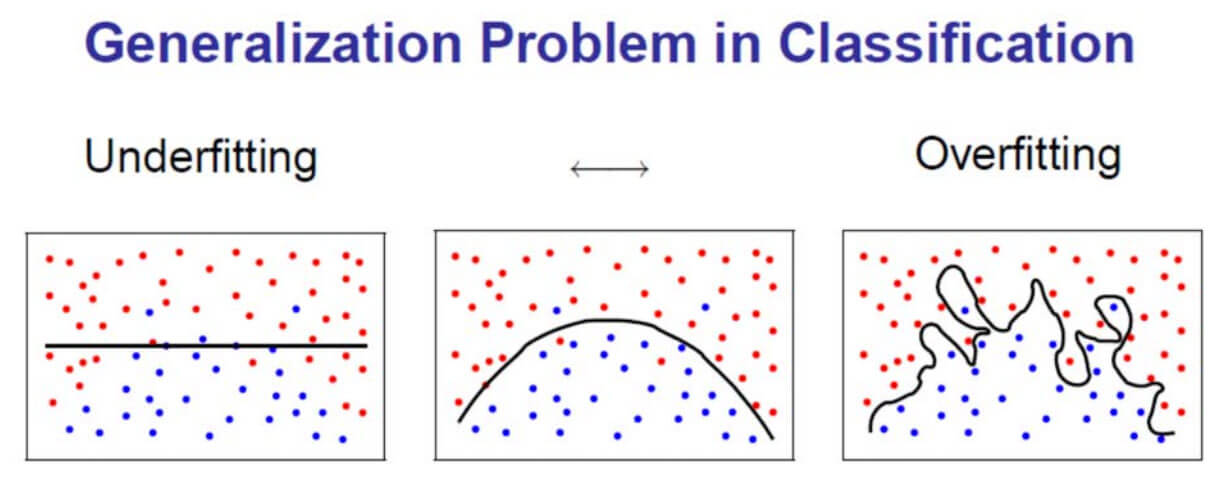
\includegraphics[scale=0.3]{overfitting.jpg}
\caption{Underfitting (left) and overfitting (right) of a classification model (solid black line) for the same dataset. Source: https://tomrobertshaw.net/2015/12/introduction-to-machine-learning-with-naive-bayes/}
\label{fitting}
\end{center}
\end{figure}

The training process for large datasets often takes the form of $k$-fold cross-validation, or simply cross-validation. In this, the training dataset is divided into $k$ random subsets. One set is used to test the others against using the classification algorithm. The process is repeated $k$ times, and the average classification results are calculated and used to determine the measures of accuracy (see below) are calculated \cite{kohavi1995study}. The number of folds in cross-validation is important, as each subset needs to have enough variety within it to contribute meaningfully to the process - if it is too pure relative to the other subsets, the subset reacts differently towards the testing data subset in an adverse manner, which lowers the overall accuracy of the process. This is more likely to occur with a high $k$-value. If the $k$-value is too low, the cross-validation is not repeated enough times for the final average to be representative of the original dataset. Both cases cause the performance of the classification model produced by the cross-validation to deteriorate.

\subsection{Information theory}

To start classification, it is necessary to select features through which to express the original data. Determining the best set of features requires the use of information theory. For a given discrete random variable (in this case a data feature $X$), its information entropy, $H(X)$, is defined as a measure of the amount of information needed to describe the variable and the average information required to describe the variable \cite{bennasar2015feature}. It is defined as:

\begin{equation}
H(X)=-\sum_{x \in X}{P(x)\textrm{log}_{2}P(x)}
\end{equation}

where $P(x)$ is the probability that $X = x$ (a.k.a. the probability mass function). From this equation, one can deduce that $0 \leqslant H(X) \leqslant 1$. The condition entropy, of a feature $X$ given another feature $Y$, is similarly defined as:

\begin{equation}
H(X|Y)=-\sum_{y \in Y}{P(y)\sum_{x \in X}{P(x|y)\textrm{log}_{2}P(x|y)}}
\end{equation}

where $P(y)$ is the probability that $Y = y$ and $P(x|y)$ is the probability of $X = x$ given $Y = y$. The joint entropy of two variables $X$ and $Y$ is:

\begin{equation}
H(X,Y)=-\sum_{x \in X}\sum_{y \in Y}{P(x,y)\textrm{log}_{2}P(x,y)}
\end{equation}

where $P(x,y)$ is the joint probability of $x$ and $y$ occuring \cite{bennasar2015feature}. In this project's datasets, the variable $Y$ takes the form of the class label \cite{lyon2016fifty}, which is the variable of most interest in this dataset, as it is the output variable in this project. The mutual information (MI), $I(X;Y)$, between $X$ and $Y$ is the amount of information that can be determined through one variable about another and can be defined in terms of their entropies by:

\begin{equation}
I(X;Y)= H(X) - H(X|Y)
\end{equation}

If two variables $X$ and $Y$ are statistically independent, their MI is zero. From this one can finally define the joint mutual information (JMI) of other features to a given feature $X$:

\begin{equation}
JMI(X)= \sum_{X' \in F} I(X,X';Y)
\end{equation}

where $F$ is the set of features other than $X$ \cite{lyon2016fifty} and $I(X,X';Y)$ is defined as \cite{bennasar2015feature}:
\begin{equation}
I(X,X';Y) = I(X;Y|X')+I(X';Y)
\end{equation}

\subsection{Classification measurements}

The results of binary classification come in the form of the true positive ($TP$), false positive ($FP$), true negative ($TN$) and false negative ($FN$) totals, which denote the number of each class (positive or negative) that were classified correctly or incorrectly, respectively, by the classifier. These can be summarised as the so-called confusion matrix \cite{kubat1998machine}, $C$:

\[
C =
  \begin{bmatrix}
    TP & FP \\
    FN & TN
  \end{bmatrix}
\]
These numbers are important, as they define ta number of measures of accuracy \cite{lyon2016fifty} used in this project. The recall (or true positive rate), $R$, is the fraction of all true positives that were classified correctly:

\begin{equation}
R = \frac{TP}{TP + FN}
\label{recall}
\end{equation}

The precision, $P$, is the fraction of the data points classified as positives which are actually positives:

\begin{equation}
P = \frac{TP}{TP + FP}
\label{prec}
\end{equation}

The specificity, $S$, is the negative analogue to the recall, as it is the fraction of real negatives that are correctly classified:

\begin{equation}
S = \frac{TN}{TN + FP}
\label{spec}
\end{equation}

The false positive rate, $FPR$, is equal to $1 - S$, as it is the fraction of negatives incorrectly classified as positives:

\begin{equation}
FPR = \frac{FP}{FP + TN}
\label{FPR}
\end{equation}

From these definitions, it can be deduced that $R$, $FPR$ and $S$ are all independent of class imbalance - the relative difference between the numbers of positive and negative data in a given dataset.
\paragraph{}
These are used, in turn, to define more acrruacy measures. The geometric mean, or G-mean, $G$, is a measure which is sensitive to fractional misclassification, rather that the absolute value of the elements of the confusion matrix themselves, \cite{kubat1998machine} and is defined as:

\begin{equation}
G = \sqrt{R \times S}
\label{gmean}
\end{equation}

Therefore, for datasets with a large class imbalance, such as the datasets used in this project, the G-mean is particularly sensitive to misclassification in the smaller class, in this case the pulsars. The F-score, $F$, is a measure that accounts for both precision and recall, and therefore is sensitive to overall fractional errors in the model for classifying positives:

\begin{equation}
F = 2 \times \frac{P \times R}{P+R}
\label{fscore}
\end{equation}

Finally, the overall accuracy, $A$, is the fraction of all of the data points which are correctly classified:

\begin{equation}
A = \frac{TP+TN}{TP+FP+TN+FN}
\label{accu}
\end{equation}

For datasets from radio astronomy surveys, which contain many more negatives (noise) than positives (astronomical objects, such as pulsars and FRBs), the accuracy is not particularly sensitive towards the classifier's performance on the positive class. This is problematic since, in this project, the performance on the smaller class is more important regarding the final objective (discovering astronomical sources). Therefore, the recall of the data was of greater interest than the accuracy for this project.
\paragraph{}
Receiver operator characteristic (ROC) curves (see Figure \ref{rocAll}) are a useful and widely-applied method for visualising the performance of a binary classifier algorithm. They are 2D plots of recall ($y$-axis) against false positive rate ($x$-axis), and thus are independent of class imbalance. The curves are generated by varying the threshold above which data points are classified as positives/anomalous objects. For supervised classifiers, the threshold is determined by the probability score. For unsupervised classifiers, it is based on the anomaly score of data. Due to the variation in the threshold, there will be a point for all algorithms where the threshold for labelling points as non-negative is maximally strict, in which case all points are classified as negative ($R = TPR = 0$). There will also be a corresponding point at which the threshold is maximally generous and classifies everything as non-negative ($R = TPR = 1$). Therefore, all curves must start at (0,0) and end at (1,1).
\paragraph{}
ROC curves allow for a comparison of a classifier results with that of a purely random process, which follows the line $R = FPR$ in an ROC curve - each point has an equal and independent chance of being classified correctly or otherwise. A perfect classification, in which all data are correctly labelled, independent of the threshold value (i.e. $R = 1$, $FPR = 0$), would be a step function, with the step at $FPR = 0$ going from $R = 0$ to $R = 1$. The relative performance of algorithms can be seen visually by examining how close the curves are to the ideal curve, or, more analytically, by calculating the area under the curve (AUC). The ideal classifier has an AUC of 1 (the entire area covered by the axes) and the purely random classifier has an AUC of 0.5. The better a classifier's performance, the greater its AUC score.
\paragraph{}
Precision-recall curves (see Figure \ref{precVsRecCutoff}) are also useful. This is because the project focuses primarily on the detection of non-noise class objects. The precision is therefore of interest. Its sensitivity to class imbalance is used here, to help determine how high the user should make the threshold probability/anomaly score for a given classifier to classify a data point as non-negative. As with the ROC curve, the curve is generated by varying this threshold. The curve allows the user to determine how high the recall of a classifier (how generous the threshold score) can be without this leading to an excessively low precision value. The curve for a given classifier will start at ($R$,$P$) = (0,1) and end at (1,0) as the threshold changes from being maximally strict to maximally generous. A perfect classifier would generate a curve in the form of a step function with the step at $R=1$.

\subsection{Classifier algorithms}
\subsubsection{Supervised learning algorithms}
The algorithms used in this project covered a wide range of properties and behaviours, since the aim of the project was to improve, and therefore prioritise, overall classifier performance in a general scenario, rather than focus on particular properties of certain algorithms. The ScikitLearn algorithm modules used \cite{scikit-learn} were:
\begin{itemize}
\item CART$\_$tree: Decision tree (DT) module. A decision tree separates data into different nodes depending on feature values (a process known as "recursive partitioning"), then splits the data within those nodes into more nodes and so on until the nodes contain data which best resembles the desired outputs. Small trees are easy to interpret visually as a series of logical steps (see Figure \ref{iTree} in the Appendix) and trees in general are fast to construct compared to other types of logarithms, even for large datasets, and require little preparation of data. However, they are prone to overfitting and are often noisy \cite{friedman2001elements}.

\begin{figure}[h!]
\begin{center}
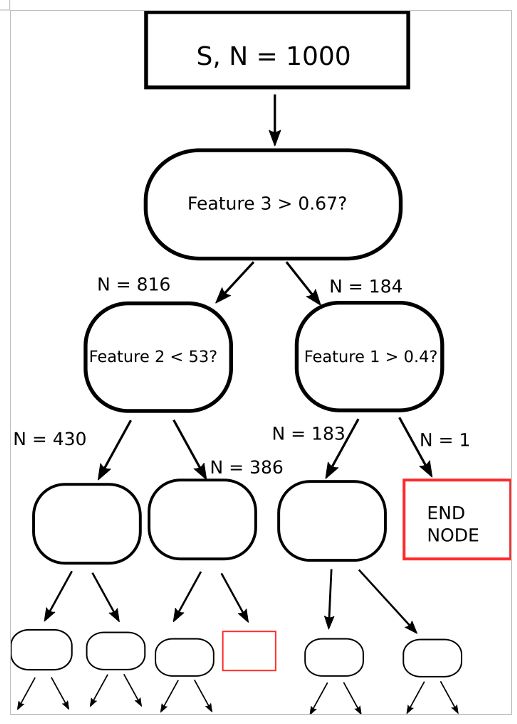
\includegraphics[scale=0.7]{itree.png}
\caption{Diagram of a decision tree, in this case an isolation tree. The end nodes are denoted by red square boxes.}
\label{iTree}
\end{center}
\end{figure}

\item Multi-layer Perceptron (MLP): An artificial neural net (ANN), which takes the set of features as an input layer of neurons, with each neuron representing a feature, and generates the output neuron layer through one or more hidden layers in between. Hidden layers each have an unknown number of neurons. Each neuron in a given layer connects to all neurons in the next layer with an individual weighting \cite{lisboa1993techniques}. The optimization is performed by reducing the errors when data points are passed along the connections. ANNs are less prone to overfitting than decision trees and can model more arbitrary functions to produce greater accuracy, but are computationally more expensive.

\iffalse
\begin{figure}[h!]
\begin{center}
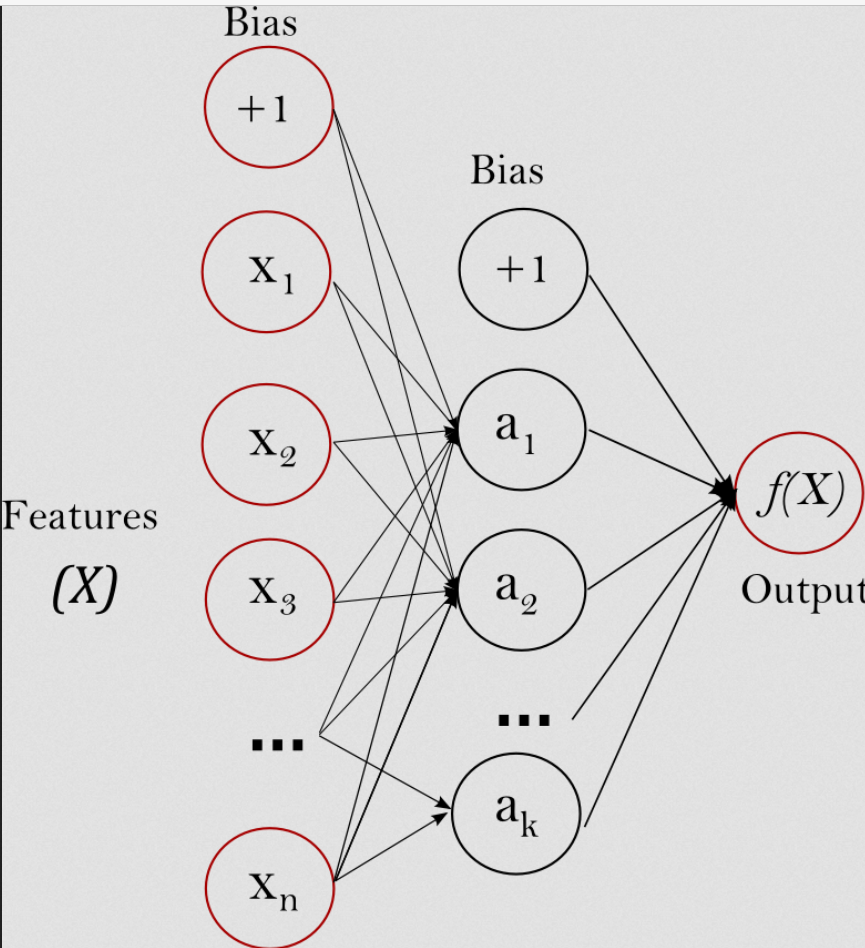
\includegraphics[scale=0.3]{multilayerperceptron_network.png}
\caption{Diagram of an ANN (specifically the MLP) with one hidden layer. Source: http://scikit-learn.org/stable/modules/neural$\_$networks$\_$supervised.html}
\label{MLPdiagram}
\end{center}
\end{figure}
\fi

\item NaiveBayes (NB): Uses a simple approach in which the data features are assumed to be conditionally independent, given the class, and then applies Bayes' theorem to calculate the probability of each class given the features. \cite{john1995estimating}. A variation on this classifier is the Gaussian NB classifier, in which the data for each class is assumed to be distributed according to a Gaussian probability distribution for each feature. Gaussian NB \cite{scikit-learn} was used for plotting FRB data.

\item Support Vector Machine (SVM): Carries out a mapping in the $N$-dimensional feature space as described earlier, but is designed for datasets in which it is impossible to separate classes using a linear boundary to represent the model(``non-separable" data). It defines a non-linear boundary between classes by using a transformed version of the feature space, in which a linear boundary is created. The algorithm defines a band around the hyperplane, with a margin $M$ defined as the distance from the hyperplane to the limit of the band on either side \cite{friedman2001elements}. The perfect margin should have all points of one class on one side of it and all those of the other class on the other side. The points not in the correct regions have displacement vectors $\xi_{i}^{*}$ (see Figure \ref{svm}). The algorithm optimizes the model by maximising $M$ subject to a maximum value of the sum of all $\xi_{i}^{*}$.

\begin{figure}[h!]
\begin{center}
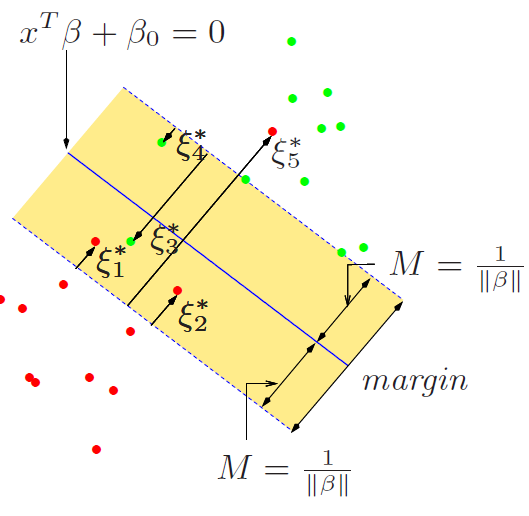
\includegraphics[scale=0.5]{svm.png}
\caption{SVM margin band (dashed line), with $\xi_{i}^{*}$ being the displacement vectors (in black) of each point from the correct region of the space. The model is the central blue line. Source: \cite{friedman2001elements}}
\label{svm}
\end{center}
\end{figure}

\item Random Forest: An ensemble algorithm (which uses several individual algorithms) that compares a group of different decision trees to optimise the training set, through a prediction that averages the predictions of all trees, which are weighted individually, in the neighbourhood of a data point \cite{friedman2001elements}. Random forests are less susceptible to overfitting than individual trees.

\item AdaBoost: An ensemble algorithm which ``boosts", or improves, the performance of a group of classifiers, some of which are little better than random guesses, known as ``weak classifiers", by comparing the accuracy of each classifier to calculate a weight. The final predictive model is then a sum of the models of the individual classifiers multiplied by their individual weights. More accurate classifiers have a greater weight \cite{friedman2001elements}.
\end{itemize}

Additionally, the Gaussian-Hellenger Very Fast Decision Tree (GH-VFDT), as detailed by Lyon et al. \cite{lyon2016fifty}, was used to confirm the results of Table 11 in the same paper, but was then discarded.

\subsubsection{Unsupervised learning algorithms}
The following unsupervised learning algorithms were used in this project but were not considered important to the final outcome. Therefore, they will not be discussed in detail:
\begin{itemize}
\item One-class SVM: Adaptation of SVM for anomaly detection - it only trains on one class. This is done by transforming the feature space using a kernel function, then treating the origin of this space as the only member of the second class. Standard SVM procedure is then followed \cite{manevitz2001one}
\item Elliptic Envelope: Assumes the negatives are distributed  in feature space as a multivariate Gaussian and fits the means and standard deviations to the data. Any outliers from this model are classified as anomalies/non-negatives.
\item Principal Component Analysis (PCA): Similar in concept to the elliptic envelope. For a dataset of $n$ features, a PCA classifier finds $q < n$ orthonormal axes such that the variance of the data when projected onto this lower-dimensional feature space, is maximal. These $q$ features are referred to as the principal components. The $q$ features are defined as the eigenvectors of the sample covariance matrix, which measures the data's variance from the sample mean over the original $n$-dimensional feature space,  with the highest eigenvalues \cite{tipping1999mixtures}.
\end{itemize}

The main unsupervised learning algorithm used in this project, however, was the Isolation Forest (IF) \cite{liu2008isolation}. This is an ensemble algorithm which takes the average result from $t$ individual isolation trees (iTrees), in the same manner as a random forest. An example of which is shown in Figure \ref{iTree}, for each one of $n$ data points being analysed. An iTree behaves in the same manner as a regular decision tree, by separating data points using decision boundaries, based upon the available features, at each node (except for the end nodes). The difference comes from the fact that unsupervised learning output is not restricted to two classes. An iTree instead continues running until a node has been created for each data point or a set limiting number of branching steps is reached, so that overall, all data points are in an "external" or "end" node (a node that no longer branches out). The number of recursive partitions required to separate a given data point, $x$, into its own node is known as the "path length", $h(x)$. The path length is recorded for each tree, and the results for all $t$ trees are used to generate an isolation score, $s(x,n)$, for the forest for each point. This isolation score is defined as:

\begin{equation}
s(x,n) = 2^{-\frac{E(h(x))}{c(n)}}
\label{itreescore}
\end{equation}

where $E(h(x))$ is the expectation value of $h(x)$ over $t$ results and:

\begin{equation}
c(n) = 2H(n − 1) − (2(n − 1)/n)
\label{plmean}
\end{equation}

is defined as the mean path length of unsuccessful searches in binary search trees \cite{liu2008isolation} (such as the supervised learning trees mentioned earlier). The isolation score is normalised - if a point is isolated into an external node immediately ($E(h(x)) = 0$), $s(x) = 1$, while $s(x) \to 0$ if $ E(h(x)) \to n-1 $, i.e. if $x$ must be separated point-by-point from the other data or the height limit of the tree is reached. The advantage of using this classifier is that it can split the training data into subsamples containing $\psi$ randomly-selected datapoints, and train on these subsamples instead of the entire dataset. This is useful for larger datasets with a class which can be accurately represented with a much smaller subset, such as the noise present in radio astronomy. Thus subsampling, if the subsample is of the correct size, saves time and requires less computing power, while sacrificing very little information for the model being optimised during the training stage.

\section{Methodology and results}
\subsection{Pulsars}
The algorithms detailed in Table 11 of Lyon et al. \cite{lyon2016fifty} were run on all three datasets to test the reproducibility of the results. The results were reproduced successfully. Then, with the exception of the GH-VFDT, those algorithms (or their ScikitLearn equivalents) were used as classifiers for the pulsar data, along with the AdaBoost and Random Forest ensemble algorithms. Feature selection was achieved using JMI maximisation (see Section 4.1). Two feature sets were compared:

\begin{itemize}
\item Lyon features: Detailed by Lyon et al.\cite{lyon2016fifty}, this is a set of 8 features consisting of 4 statistical measures - the mean, standard deviation, skewness and kurtosis, which are the first, second, third and fourth statistical moments, respectively - applied to both the pulse profile and DM-SNR curve.
\item Thornton features: Detailed by Thornton \cite{thornton2013high}, this is the set of 22 features originally implemented for the Stuttgart Neural Network Simulator (SNNS), including the period and dispersion measure as well as how the pulse profile shape matches to various curves, such as Gaussians.
\end{itemize}

The Lyon feature was judged to be better overall via averaging the ranks of the JMI score for the individual features over the 3 datasets. It was then combined with the period, which was needed to separate the pulsars into MSPs and non-MSPs, and class values, which were designated as outputs, allowing for comparison of the cross-validation and test results with the real values.

\begin{figure}[h!]
\begin{center}
\includegraphics[scale=0.5]{HTRU2_noise(b)_psr(g)_dm_mean_vs_stddev.png}
\caption{Raw HTRU2 data: pulsars (green), including MSPs, compared to noise (blue)}
\label{HTRU2noisepsr}
\end{center}
\end{figure}

\paragraph{}
To check the suitability of the simulated pulsar data and look for relations between features, the data was manipulated to visualise the data in WEKA via plots such as Figures \ref{HTRU2noisepsr} and \ref{DMMeanStddevBadvsMSP}. When the simulated data was declared viable for classification, a comment was added to classified MSPs, allowing them to be distinguished from other real pulsars as well as the simulated MSPs. Using this comment, the real MSPs were removed from the HTRU2 data and placed into a separate ARFF file, which would be used as the testing dataset during classification, with the remaining data being used as the training set.

\begin{figure}[h!]
\begin{center}
\includegraphics[scale=0.5]{HTRU2_msp(b)_sim_r3(g)_dm_mean_vs_stddev.png}
\caption{Unrealistic simulated MSP data (green) compared to HTRU2 MSPs (blue)}
\label{DMMeanStddevBadvsMSP}
\end{center}
\end{figure}

When creating the simulated MSP data, the way in which the data was processed was very important with regard to how realistic it appeared in the feature space compared with real MSPs. Any datasets which had not been generated in the exact same way as the original HTRU2 data were easily distinguishable from the real data, particularly in their DM-SNR curve features. This is shown in Figure \ref{DMMeanStddevBadvsMSP}, where most simulated MSPs can clearly be separated from real MSPs by a line bisecting the lines followed by each group. These differences adversely affect the model being used to classify real MSPs. The final simulated dataset, consisting of 744 simulated MSPs, did not deviate from the feature trends shown by the real pulsars upon visual inspection, and, within those trends, closely aligns with the regions occupied mostly by the real MSPs (see Figure \ref{HTRU2simr5} in the Appendix). Consequently, they were assessed to be realistic in the Lyon feature space.
\paragraph{}
For classifying the real MSPs, the  training dataset, containing everything except the real MSPs, underwent cross-validation, with the noise being class-0 and all remaining pulsars (including simulated examples, where relevant) being class-1, with the number of folds set at $k$ = 5. The real MSPs were then used as the testing set, using the model created by the cross-validation of the training data. Since the testing set was made up purely of class-1 objects (the real MSPs), the accuracy and recall of algorithms applied to that set are exactly the same by definition. This was done as part of the overall emphasis on the pulsars in the data.
\paragraph{}
\begin{table}[h!]
\centering
\resizebox{\columnwidth}{!}{%
\begin{tabular}{|l|l|l|l|}
\hline
\textbf{Classifier} & \textbf{$R$ for HTRU2 data} & \textbf{$R$ for HTRU2 + sim.} & \textbf{$R$ for corrected HTRU2} \\ \hline
CART\_tree          & 0.301 $\pm$ 0.042                     & 0.594 $\pm$ 0.023               & 0.698 $\pm$ 0.026 \\ \hline
MLP                 & 0.383 $\pm$ 0.027                     & 0.603 $\pm$ 0.012               & 0.695 $\pm$ 0.020 \\ \hline
NaiveBayes        & 0.380 $\pm$ 0.000                     & 0.465 $\pm$ 0.000               & 0.561 $\pm$ 0.000 \\ \hline
SVM                 & 0.487 $\pm$ 0.013                     & 0.682 $\pm$ 0.008               & 0.786 $\pm$ 0.008 \\ \hline
Random Forest      & 0.293 $\pm$ 0.058                     & 0.563 $\pm$ 0.039               & 0.698 $\pm$ 0.008 \\ \hline
AdaBoost            & 0.358 $\pm$ 0.016                     & 0.558 $\pm$ 0.008               & 0.660 $\pm$ 0.010 \\ \hline
\end{tabular}
}
\caption{Recall on HTRU2 MSPs (class 1) using the HTRU2 noise (class 0) and non-MSPs (class 1) as training data}
\label{HTRU2}
\end{table}

A test of significance was carried out on the HTRU2 results generated before and after added the simulated MSPs to the training data, in the form of a student's t-test. A student's t-test was chosen as it controls for sample sizes, which is important, given the differences in pulsars numbers before and after adding the simulated MSPs. This generates a result, known as the p-value, using the two results and their respective standard deviations. The threshold p-value was chosen as p$_{thres}$ = 0.05, which is a typical value and indicates that rejection of the null hypothesis is acceptable to a maximum error of 5$\%$ , with the p-value representing the actual calculated error. Hence, if the significance test generates a p-value less than p$_{thres}$, the null hypothesis is rejected and the difference between results is significant \cite{friedman2001elements}. Having used HTRU2 as a dataset to optimize the simulated data, the simulated data was added to HTRU1 and the algorithms were then applied to the resulting dataset. After adding simulated MSPs to the training set, the recall on HTRU2 increased significantly compared with using just raw observational data (see Table \ref{HTRU2}), while the recall on HTRU1 did not change significantly (see Table \ref{HTRU1}).

\begin{table}[]
\centering
\begin{tabular}{|l|l|l|}
\hline
\textbf{Classifier} & \textbf{$R$ for HTRU1 data} & \textbf{$R$ for HTRU1 + simulated data} \\ \hline
CART\_tree          & 0.819 $\pm$ 0.040                & 0.859 $\pm$ 0.025                                 \\ \hline
MLP                 & 0.816 $\pm$ 0.012                & 0.854 $\pm$ 0.034                                 \\ \hline
NaiveBayes        & 0.811 $\pm$ 0.000                & 0.824 $\pm$ 0.000                                 \\ \hline
SVM                 & 0.981 $\pm$ 0.007                & 0.986 $\pm$ 0.000                                 \\ \hline
Random Forest      & 0.822 $\pm$ 0.015                & 0.846 $\pm$ 0.039                                 \\ \hline
AdaBoost            & 0.789 $\pm$ 0.028                & 0.792 $\pm$ 0.008                                 \\ \hline
\end{tabular}
\caption{Recall on HTRU1 MSPs (class 1) using the HTRU1 noise (class 0) and non-MSPs (class 1) as training data}
\label{HTRU1}
\end{table}

\paragraph{}
A program was written that uses the combined HTRU2 and simulated training dataset to determine the effect of varying the MSP cutoff period threshold, $P_{MSP}$, on the MSP recall using the new definition. This was carried out by entering a quantity and range of $P_{MSP}$ values as arguments, then plotting the mean recalls against $P_{MSP}$, with error bars, for each individual classifier. The variation in definition was applied to real HTRU2 pulsars only. This was carried out for both the newly-defined MSPs and all pulsars, as a reference. The results are shown in Figure \ref{allnoiseacc} and show that the recall on real MSPs, as defined by the threshold, is not significantly affected by the exact position of the threshold.

\begin{figure}[h!]
\begin{center}
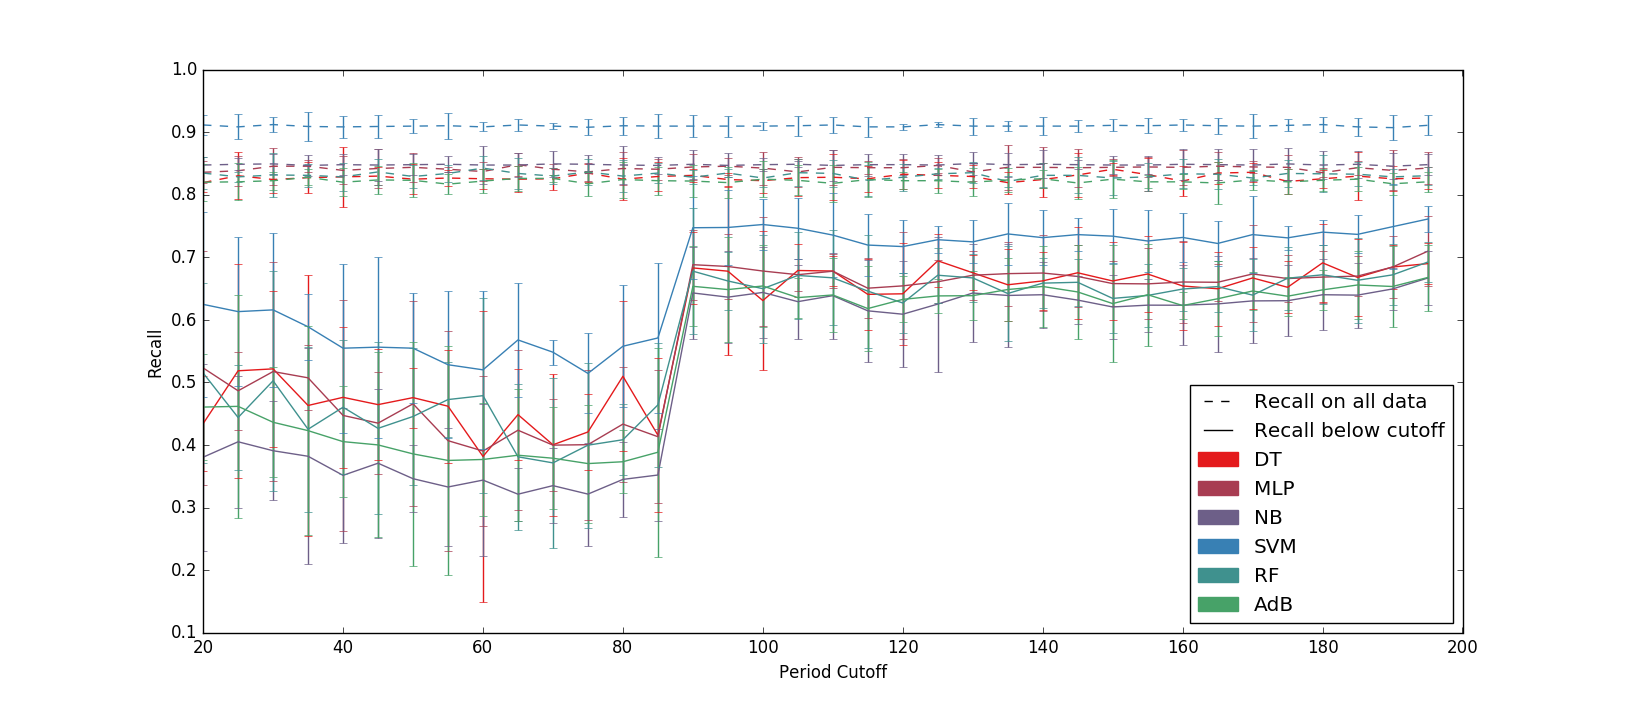
\includegraphics[scale=0.3]{acc_vs_period_v2_zoom.png}
\caption{Recall on HTRU2 MSPs for variation in the MSP cutoff period}
\label{allnoiseacc}
\end{center}
\end{figure}

A final set of programs was written such that circa 90$\%$ of noise below $P_{MSP}$ was taken out of the training set. This did not significantly affect the classification results on the resulting training dataset nor on those for the MSP testing dataset.
\paragraph{}

%To check if the datasets from Lyon et al. (2016) used in this project have an influence on the classification algorithms (i.e. the algorithms overfitted on these sets), the data from which the datasets were extracted, which was stored on a separate GPU at Jodrell Bank, was processed using PulsarFeatureLab. The data was then compared with the ATNF pulsar catalogue \cite{}, using maximum tolerance limits of 1$\deg$ on both the right ascension and declination, 10 ms on the period and 20 cm$^{-3}$pc on the DM. The dataset of successfully-matched observations was extracted together with the catalogue index of the real pulsar, before any repeated-index data was removed, leaving a dataset composed of 951 separate known pulsars. This was then combined with the noise data. Just as before, the supervised classifiers  were


\subsection{FRBs}
During feature selection, the most useful features for distinguishing FRBs were the SNR, the boxcar width and the DM. This is not surprising, as these are the defining features of FRBs. The other features examined the number of nearest-neighbour data points for a given data point for different time limits on the definition of nearest-neighbours. These intervals were on the order of a few seconds of observation time. The reasoning behind this was that, because of the transient nature of FRBs, they may be more likely to be isolated points in feature space, while terrestrial noise tends to arrive in groups of detections at similar times. However, their JMI ranks varied significantly between datasets and individual runs, due to their JMI values being very small and subject to random fluctuations. Therefore, only the SNR, DM and boxcar width were taken forward as useful features.
\paragraph{}
The classifier evaluation programmes used with the pulsar datasets were updated and added to, in order to use the new format of data (.dat files, as opposed to the .arff format previously employed with pulsars) and the unsupervised algorithms. The results were then displayed visually as ROC curves (one for each classifier), as shown in Figure \ref{rocAll}, with a corresponding value of the AUC also calculated for each curve (see Table \ref{FRBauc}). The Isolation Forest classifier, which is the best performing unsupervised classifier, is plotted in both panels for comparison with the supervised (right-hand panel) and other unsupervised (left-hand panel) classifiers.

\begin{table}[]
\centering
\begin{tabular}{|l|l|}
\hline
\textbf{Classifier} & \textbf{AUC value for FRB data} 	\\ \hline
CART\_tree          & 0.807 $\pm$ 0.078            		\\ \hline
MLP                 & 0.999 $\pm$ 0.001            		\\ \hline
NaiveBayes        	& 0.990 $\pm$ 0.008           		\\ \hline
SVM                 & 0.982 $\pm$ 0.035              	\\ \hline
Random Forest      	& 0.928 $\pm$ 0.059              	\\ \hline
AdaBoost            & 0.996 $\pm$ 0.009              	\\ \hline
Isolation Forest   	& 0.990 $\pm$ 0.009              	\\ \hline
PCA                 & 0.961 $\pm$ 0.042              	\\ \hline
One-class SVM       & 0.958 $\pm$ 0.085              	\\ \hline
Elliptic Envelope   & 0.057 $\pm$ 0.003					\\ \hline
\end{tabular}
\caption{AUC values for FRB dataset.}
\label{FRBauc}
\end{table}

\begin{figure}[h!]
\begin{center}
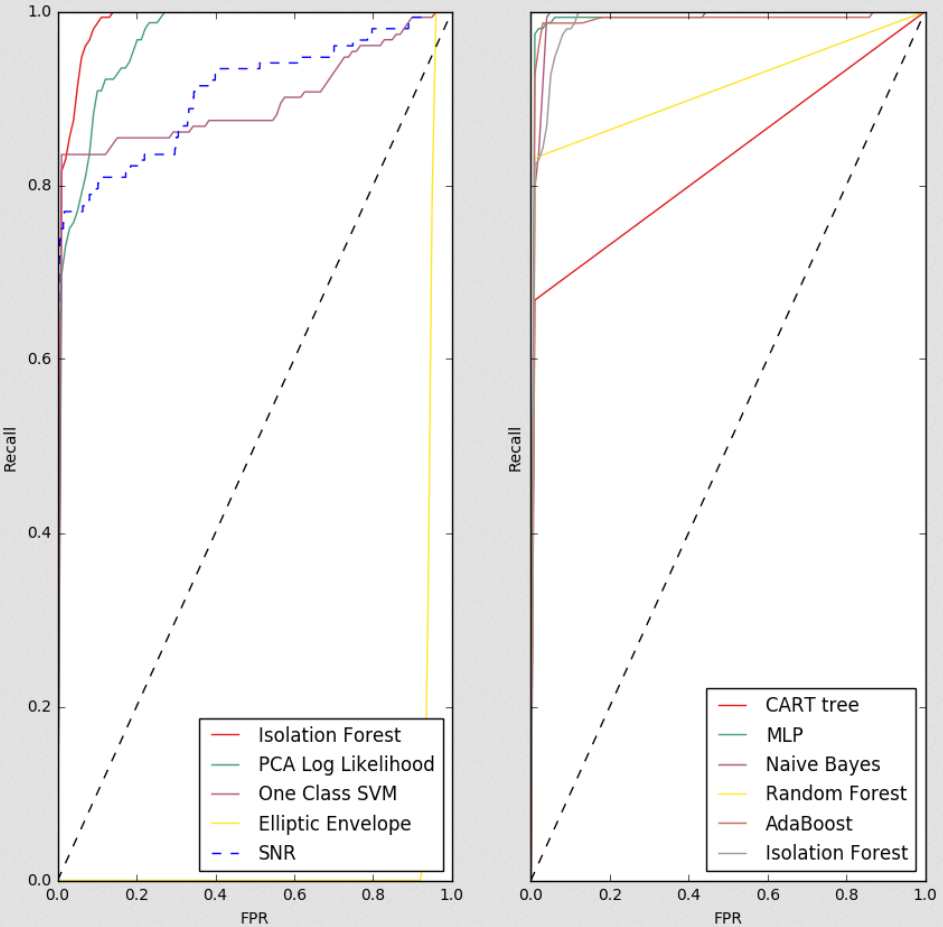
\includegraphics[scale=0.5]{2roc_frb.png}
\caption{ROC curve for FRB data of supervised (R) and unsupervised (L) classifiers, with Isolation Forest in both figures. The SNR has been included as an additional reference for the suitability of classifiers}
\label{rocAll}
\end{center}
\end{figure}


Having established Isolation Forest as the most promising unsupervised classifier, a plot of precision against recall was created (see Figure \ref{precVsRecCutoff}). Isolation Forest is plotted twice, the second time after cutting out all data points with DM $<$ 500 cm$^{-3}$pc, alongside Random Forest, AdaBoost and NaiveBayes. After applying the cutoff, the performance of  Isolation Forest improves such that it begins to outperform NaiveBayes at higher recall values in terms of precision, although it remains inferior to the other supervised classifiers.
\paragraph{}
To visualise the behaviour of the classifiers and their subsequent decision boundaries, contour plots of the data in the SNR vs. DM plane were created, with each axis scaled such that the data have zero mean and unit variance for each feature. The results are plotted in Figure \ref{frbContour}. The lighter regions represent areas of (2D) feature space in which anomalous (non-noise) data is determined to be prevalent by that particular classifier. Of the unsupervised classifiers only Isolation Forest and one-class SVM are able to separate FRBs and noise adequately, while the only supervised classifier to do so  without overfitting on FRBs is the Gaussian NaiveBayes. The other supervised classifiers (which require both classes in the training data) effectively "learn" that the (simulated) FRBs have a small DM range compared with the noise data. Some classifiers also make use of the fact that the FRBs also have a lower limit on their SNRs relative to the noise.

\begin{figure}[h!]
\begin{center}
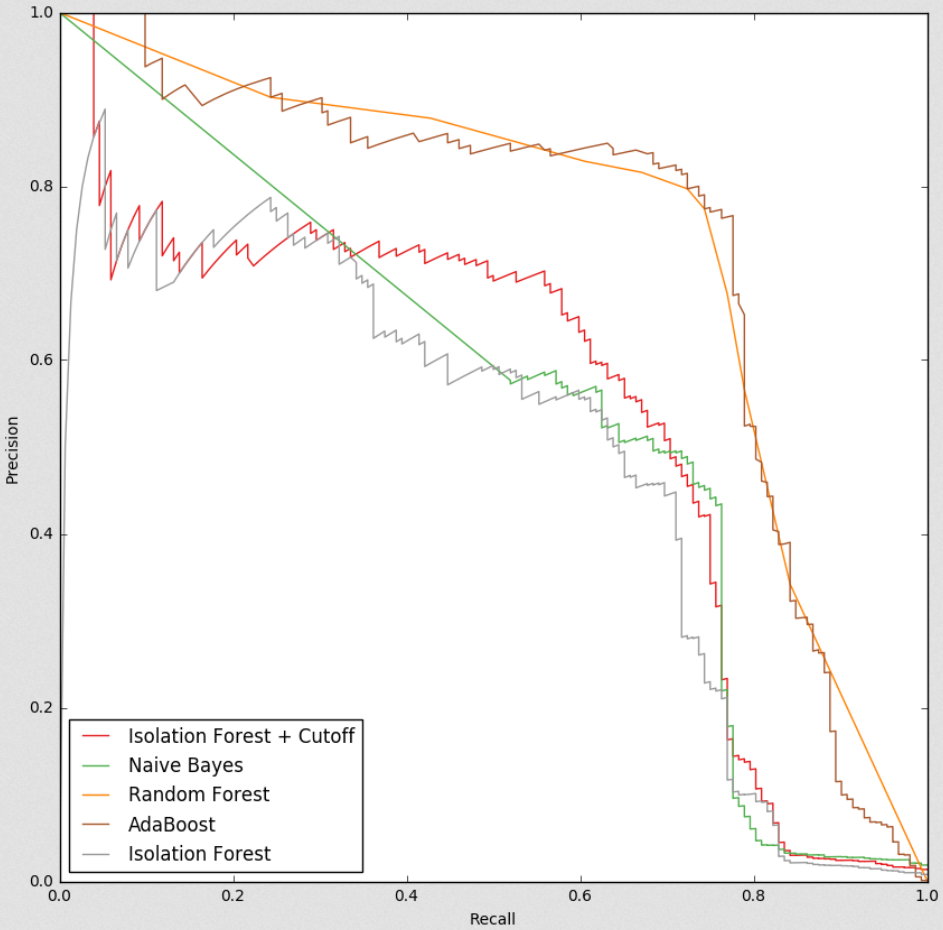
\includegraphics[scale=0.4]{prec_recall_cutoff.png}
\caption{FRB data precision-recall plot of Isolation Forest (with and without cutting out all points with DM $<$ 500 cm$^{-3}$pc, both ensemble supervised classifiers and NaiveBayes}
\label{precVsRecCutoff}
\end{center}
\end{figure}

\begin{figure}[h!]
\begin{center}
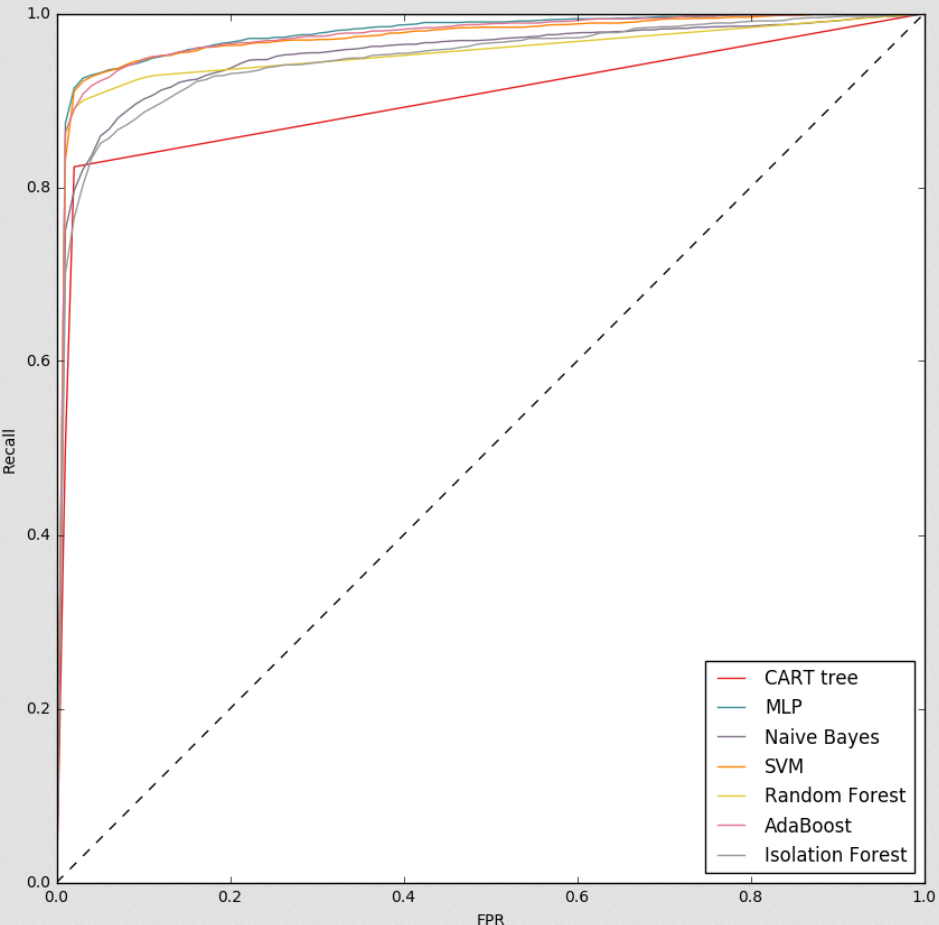
\includegraphics[scale=0.4]{htru2_roc.png}
\caption{ROC curve of Isolation Forest together with the supervised algorithms, applied to HTRU2}
\label{HTRU2roc}
\end{center}
\end{figure}

\section{Discussion of classification results}
\subsection{Pulsar results}
The Lyon feature set is better for classifying pulsars by machine learning in this project partly because there are fewer features than is the case for the Lyon features, which makes the processing less complicated and quicker (i.e., it is less prone to the so-called ``curse of dimensionality"). Secondly, they are generic statistics-based features which directly relate to existing classification techniques, as they are simply the four lowest statistical moments of two of the graphics already used by human researchers to classify objects (see Figure \ref{psrsoftsim}). By contrast, some of the Thornton features are speculative, such as  $\chi^{2}$ results of fitting the pulse profile to various models, or are insensitive to some details, such as the feature using the area under the pulse profile, which can take the same value for a very narrow, tall profile or a broad, short profile, and which therefore requires additional features to extract the details, which is more inefficient. Thirdly, the variety of pulse profiles shown by Pilia et al. \cite{pilia2016wide} indicates that speculative fittings may be even less efficient as features, since most will be redundant for any given pulsar and the pulsar may not conform adequately to any of them.

\paragraph{}
\begin{figure}[h!]
\begin{center}
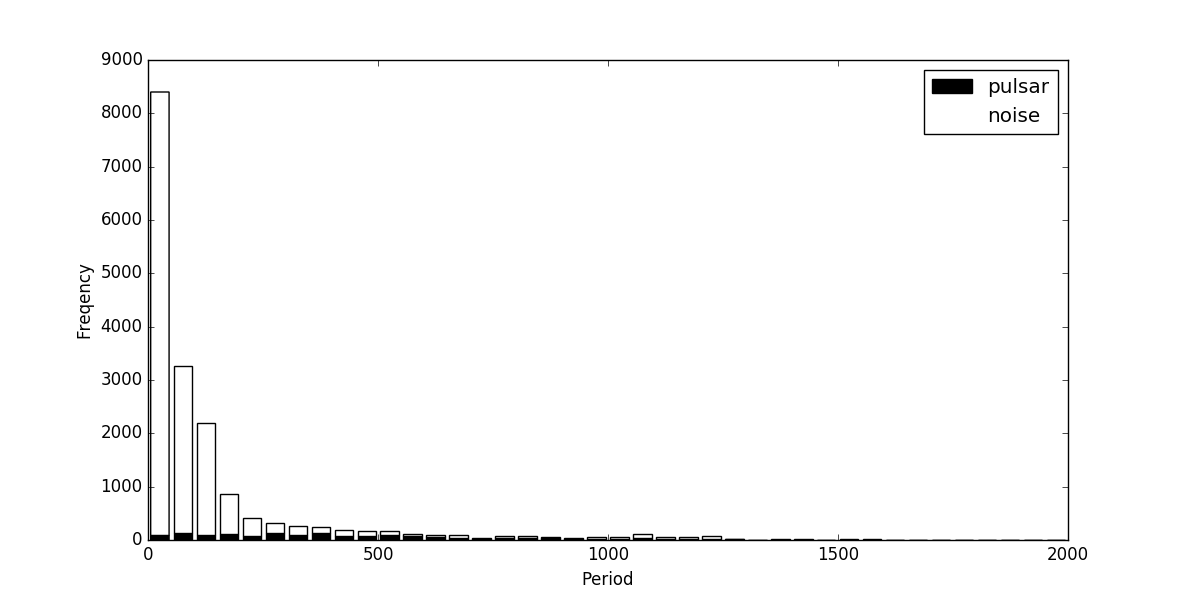
\includegraphics[scale=0.4]{pulsar_period_hist.png}
\caption{Histogram of HTRU2 noise (white) and pulsar (black) data, showing class imbalance in favour of noise data, particularly at low periods}
\label{HTRU2hist}
\end{center}
\end{figure}

The addition of simulated data clearly and significantly improves the performance of the classification algorithms on the HTRU2 data. This is not only due to the realistic appearance of the data in the feature space, but also to the impact of adding a large number (744) of simulated MSPs to the real MSP population (71), as it counters the dominance of non-millisecond pulsars within the dataset of classified pulsars, as well as noise within the full dataset (see Figure \ref{HTRU2hist}).
\paragraph{}
The performance of the NaiveBayes classifier was the poorest of the classifiers overall and the standard deviation effectively zero, which is indicative of an underlying problem. The NaiveBayes classifier assumes the features it uses to be independent of one another, which is clearly contradicted by the aforementioned trends in the data.
\paragraph{}
The performance of the SVM classifier was the best overall, which is likely due to its main strength of classifying non-separable data (see Section 2.4), of which the datasets in this project are examples (Figure \ref{HTRU2noisepsr} in the Appendix is one example of the substantial mixing of data points from both classes in HTRU2).
\paragraph{}
HTRU1 was not improved by any level of significance by the addition of the final simulated data. However, the classifiers performed very well without adding the simulated data, leaving little room for improvement. Also, had the simulated data been completely unrealistic for HTRU1, its addition would have been expected to cause the results to deteriorate.
\paragraph{}
It must be noted, however, that HTRU1 and HTRU2 were processed using different pipelines methods and codes, which may explain how two sets of data from the same survey can produce such different performance levels from the same classifier algorithms and for every one of those algorithms. HTRU1 was processed using the PEASOUP pipeline, detailed by Morello et al. \cite{morello2014spinn}, while HTRU2 was processed using PDMP by Thornton \cite{thornton2013high}. The surprisingly high significance of how exactly a dataset was processed upon the data itself had already been witnessed when processing the simulated datasets (see Section 6).
\paragraph{}
The effect of varying the period threshold for defining MSPs is not significant, which is surprising, since MSPs are very clearly defined from an astrophysical perspective (see Introduction). The increase in recall in the 80-100 ms cutoff period interval is not significant for each classifier individually, but its transcendence of every algorithm in Figure \ref{allnoiseacc} suggests it is significant overall. However, the simultaneous increase in the MSP-to-noise candidate ratio (see Figure \ref{noiseratiocutoff} in Appendix) suggests than the significance of the effect is due to the sudden appearance of pulsar data, as the period increases, which allows the classifiers to better separate the classes overall. This could also be due to localised lessening of noise dominance (class imbalance) as more pulsars are added to the MSP dataset.

\begin{figure}[h!]
\begin{center}
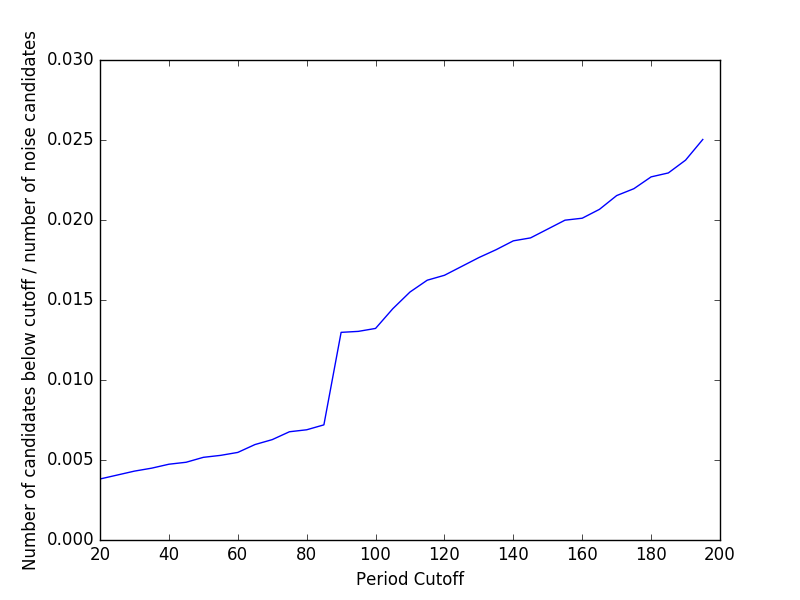
\includegraphics[scale=0.5]{noise_ratio_vs_period_cutoff_zoom.png}
\caption{Ratio of MSPs to noise candidates as a function of $P_{MSP}$}
\label{noiseratiocutoff}
\end{center}
\end{figure}

\paragraph{}
The effect of noise reduction was found to be statistically insignificant. This suggests that correctly classifying pulsars will depend more on the pulsar data rather than the noise data. Noise reduction is not particularly helpful in the context of classifying data in real time, as it requires the data to be classified beforehand. This, in turn requires data to be stored and then analysed closely. This process is not perfect, as shown in Table \ref{HTRU2}, where, for some classifiers, the misclassification of noise data as MSPs causes the classifier performance to deteriorate significantly.

\subsection{FRB results}

\begin{figure}[h!]
\begin{center}
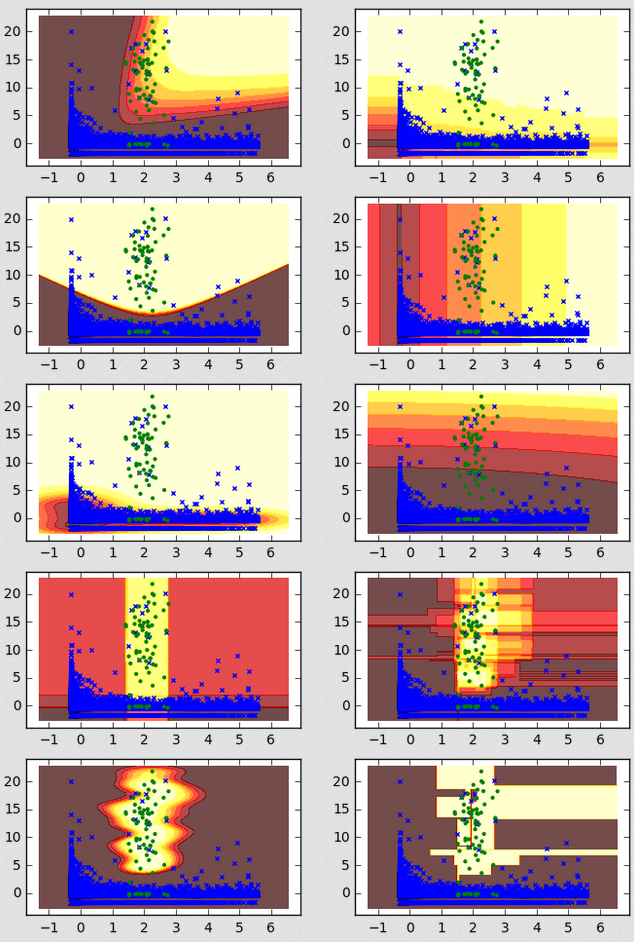
\includegraphics[scale=0.5]{classifier_contours.png}
\caption{SNR-DM contour maps of FRB data for the following classifiers (clockwise from top left): MLP, Isolation Forest (with subsamples of 8000 data points and 100 trees), Elliptic Envelope, PCA, Random Forest, CART tree, SVM, AdaBoost, one-class SVM, Gaussian NaiveBayes. }
\label{frbContour}
\end{center}
\end{figure}

As expected, the DM, boxcar width and SNR give the highest JMI scores during testing for feature selection. However, the other features, relating to the tendency of data points to cluster together in terms of the time of observation, produced small JMI scores which were subject to fluctuations in both their absolute values and rankings. This is significant, as FRBs are single-detection events that are anomalous compared to known sources of noise and hence should ideally occupy a different region in feature space. It is possible, therefore, that the feature space made available by the processing pipeline is insufficient for reliable detection of FRBs, as no features, aside from those used to originally define FRBs, were found which were of any use in classifying the data.
\paragraph{}
As shown in Table \ref{FRBauc}, the AUC values of all the classifiers (except Elliptic Envelope) are within a 3$\sigma$ threshold of each other, indicating that, for this dataset, supervised and unsupervised classifiers, in general, are equally useful. However, it should be noted that, when using a classifier algorithm, only a single point on the relevant curve is being used, as only a single threshold is employed throughout the classification process. It is therefore up to the user to compromise between a high recall and a low $FPR$. For a dataset such as the FRB dataset used in this project, the user should focus primarily on keeping the $FPR$ low. This is because the accuracy of non-negatives (FRBs in this case) is effectively unknown, due to the paucity of real examples. On the other hand, the negatives (noise) are all real observation data and exist in a number large enough to be a representative sample.
\paragraph{}
One of the major drawbacks of supervised learning is that it requires representative samples of all relevant classes (noise and FRBs). This is not a problem for the noise - there is an abundance of accurate and representative noise samples to use for training. Since this is clearly not the case for FRBs, the use of supervised classifiers cannot be justified here. In Figure \ref{frbContour}, with the exception of the Gaussian NaiveBayes, the supervised classifiers utilise the restricted (and arbitrary) range of DM values (and sometimes SNR values) in the simulated FRB population to define their decision boundaries. While this is technically desirable for a supervised classifier, it is, in reality, a sign of their unsuitability in the case of FRBs. This is because there is no indication of the simulated FRBs being representative of all possible FRB detections and there are no reliable FRB datasets, simulated or otherwise, upon which to train classifiers. This leads to a significant risk of a supervised classifier misclassifying an FRB as noise merely because the classifier has effectively overfitted on a non-representative FRB dataset. Therefore an unsupervised classifier, which only requires noise data to produce a model, should be used for screening FRB candidates.
% In some cases, they also uses the lower limit of the SNR for the FRBs. Since t, an unsupervised classifier, which only requires noise data to produce a model, should be used for screening FRB candidates. This is due to the fact that there is currently no reason to expect all future FRB detections to occur in a relatively small area of feature space. Therefore, the simulated FRB data cannot be described as representative of all FRB data. If these supervised classifiers were used, any FRBs outside these strict limits would be misclassified as noise.
\paragraph{}
Isolation Forest is the best performing unsupervised classifier overall, as shown by the left-hand ROC curve in Figure \ref{rocAll}. The others perform almost as well (within the margin of error relative to Isolation Forest), with the exception of the Elliptic Envelope algorithm, which performs far worse than even a random guess. Regarding the precision-recall curve in Figure \ref{precVsRecCutoff}, it remains competitive with NaiveBayes, the only supervised algorithm type (if Gaussian NaiveBayes is included) which does not base its decision boundaries on learning the DM limits of the simulated FRB data, as shown in Figure \ref{frbContour}. By comparing the results from Figures \ref{frbContour} and \ref{precVsRecCutoff} for the classifiers which appear in both, it is not surprising that the precision is worse for Isolation Forest and NaiveBayes, as the white areas in their contour plots include many more noise data points than those of AdaBoost and Random Forest.
\paragraph{}
Isolation Forest possesses a range of other properties which are desirable in the context of transient radio searches. Unlike some of the other unsupervised classifiers, it does not assume a particular distribution of noise data in feature space. It is computationally less complex (and therefore less expensive, and quicker, to run) than other classifiers. When training its optimisation function its complexity is of order $O(t \psi log(\psi))$, i.e. completely independent of the number of data points, in the dataset, $n$. In fact, the classifier often reaches acceptable performance levels for relatively small values of $t$ and $\psi$ \cite{liu2008isolation}. When testing the model on the dataset, the complexity is of order $O(tn log(\psi))$. Since $t$ and $\psi$ are determined by the user and initialised to fixed values before the algorithm is run, they can be regarded as constants once the algorithm starts running, so the complexity is effectively of order $O(n)$. This is less complex than for PCA ($O(n^{2})$) and both types of SVM classifier ($O(n^{2-3})$) \cite{scikit-learn}.
\paragraph{}
Isolation Forests, being an application of unsupervised learning, do not require their input data to be classified beforehand. During processing of observational data, this has the double advantage of saving time (as the processing pipeline no longer needs to classify raw data) and avoiding classification errors (such as those encountered in HTRU2 with the mislabelled "pulsars"). Isolation Forests can also be adapted for use in data streams (the continual addition of data into datasets in real-time).
\paragraph{}
The combination of these properties makes Isolation Forests a strong candidate for processing data for upcoming projects such as the SKA, in which data streaming will be common, due to its exceptionally high rate of data production (see Introduction). It would be particularly useful in transient searches as it is anomaly-based, but it also performs well for pulsar data, such as HTRU2 (see Figure \ref{HTRU2roc}), and it therefore could have applications beyond transient searches.

\section{Conclusion}
Using simulated pulsar data, if it demonstrates behaviour in feature space similar to that of observational pulsar data, does significantly improve classification using supervised-learning intelligent algorithms. For pulsars, supervised learning was highly useful due to the highly non-separable nature of the data (see Figure \ref{HTRU2noisepsr}) and to the constraints on pulsars in the feature space. This allowed for the creation and use of viable simulated pulsar data, which significantly improves performance of the supervised classifiers on pulsar data.
\paragraph{}
For fast radio bursts, there is no known representative dataset of examples. FRBs by nature are anomalous readings which are otherwise unknown. Therefore they should be searched for using unsupervised classifiers via anomaly scores. The Isolation Forest classifier was found to be the best such example.

\begin{small}
\bibliographystyle{ieeetr}
\bibliography{mphysreffinal}
\end{small}

\section{Appendix}
\subsection{Source code repository}
https://github.com/lsgos/MPhysPulsars

Contains source code, datasets, simulated data, results in .png, .ods and .txt formats, Jupyter notebooks (.ipynb) and a copy of PulsarFeatureLab. All new codes for this computer-based project were written in Python 2.7.12.

\subsection{Risk assessment}
\underline{1. Hazard identification:}
\begin{enumerate}[label=(\roman*)]
\item High computer usage and the subsequent risk of sight problems due to overexposure to screens.
\item Electrocution
\end{enumerate}
\underline{2. People at risk:}
\begin{enumerate}[label=(\roman*)]
\item MPhys participants
\item MPhys participants
\end{enumerate}
\underline{3. Risk evaluation:}
\begin{enumerate}[label=(\roman*)]
\item The risk is adequately controlled due to industry standards and user guidance regarding computer screen usage.
\item The risk is adequately controlled due to grounding and insulation of wires.
\end{enumerate}
\underline{4. Actions to be taken:}
\begin{enumerate}[label=(\roman*)]
\item Take regular breaks away from computer screens.
\item Follow standard guidelines for use of electrical equipment.
\end{enumerate}
Last reviewed: 11th May 2017 \newline
Carried out by: Alex Lisboa-Wright, Lewis Smith.

Supervisor: Michael Keith.

\subsection{Additional figures}

\begin{figure}[h!]
\begin{center}
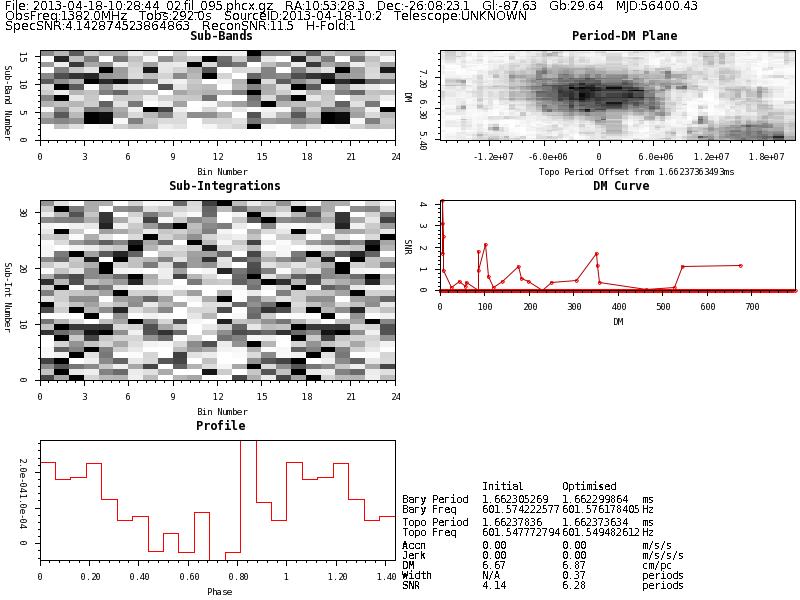
\includegraphics[scale=0.4]{2013-04-18-10_28_44_02_fil_095.png}
\caption{psrsoft image output for a non-pulsar (noise) data file}
\label{psrsoftnoise}
\end{center}
\end{figure}

\begin{figure}[h!]
\begin{center}
\includegraphics[scale=0.5]{HTRU2_msp(b)_non_msp(r)_sim_r3(g)_dm_mean_vs_skew.png}
\caption{Unrealistic simulated MSP data (green) compared to HTRU2 MSPs (blue) and non-MSPs (red)}
\label{DMMeanSkewBadvsMSPvsNon}
\end{center}
\end{figure}

\begin{figure}[h!]
\begin{center}
\includegraphics[scale=0.5]{HTRU2_msp(b)_non_msp(r)_sim_r5(g)_dm_mean_vs_skew.png}
\caption{Final (realistic) simulated MSP data (green) compared to HTRU2 MSPs (blue) and non-MSPs (red)}
\label{HTRU2simr5}
\end{center}
\end{figure}

\end{document}